
\documentclass{article}
\usepackage{polski}
\usepackage[utf8]{inputenc}
\usepackage{graphicx}

\begin{document}

\title{Specyfikacja wymagań}

\author{Mateusz Biegański, Anna Kramarska, Michał Sarzyński, Magda Suchodolska}
\maketitle

\section{Wymagania funkcjonalne}

\subsection{Diagram przypadków użycia}

\begin{center}
    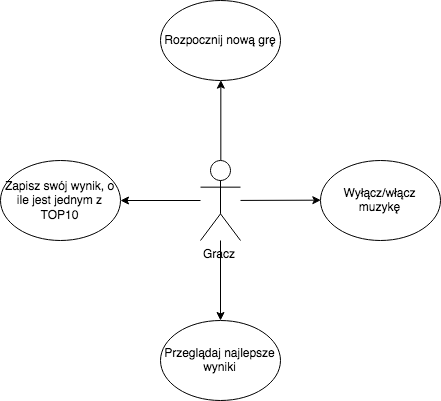
\includegraphics[scale=0.5]{use_case_diagram.png}
\end{center}

\subsection{Opis wybranych przypadków użycia}

\subsubsection{Gra}

\begin{enumerate}
    \item Gracz chce rozpoczać nową grę.
    \item Aplikacja wyświetla ekran z grą.
    \item Gracz gra w grę kładąc kolejne klocki.
    \item Gracz kończy grę nietrafiając klockiem w podstawę poprzeniego.
    \item Jeżeli wynik gracza jest jednym z 10 najlepszych, gracz zapisuje wynik.
\end{enumerate}

\subsubsection{Najlepsze wyniki}
\begin{enumerate}
    \item Gracz chce wyświetlić 'TOP 10'.
    \item Aplikacja wyświetla ekran z listą co najwyżej 10 najlepszych wyników.
\end{enumerate}

\section{Wymagania niefunkcjonalne}

\textbf{Po ukończeniu prac nad Palace 2D zakładamy spełnienie poniższych
wymagań niefunkcjonalnych:}
  \begin{itemize}
  \item Aplikacja działa na systemie Linux
  \item Poprawne działanie aplikacji nie wymaga dostępu do Internetu
  \item Poprawne działanie nie wymaga instalowania dodatkowych pakietów
  \item Rozmiar na dysku nie przekracza 300MB
  \item Rozdzielczość 800x600px
  \item Częstotliwość wyświetlania klatek: 60 klatek/sekundę
  \end{itemize}


\textbf{\newline Zakładamy że wszystkie powyższe wymagania zostaną
spełnione na maszynie o podanej specyfikacji:}
\begin{itemize}
  \item System Linux x86 64, wersja jądra 4.9
  \item CPU: Intel Core 2 Duo
  \item Karta graficzna: NVIDIA GTX 750Ti
  \item Pamięć RAM: 2GB
\end{itemize}

\end{document}
